\documentclass[aspectratio=169, 10pt]{beamer}

% ==========================================
% PACKAGES & SETUP
% ==========================================
\usepackage[utf8]{inputenc}
\usepackage[T1]{fontenc}
\usepackage{helvet}
\usepackage{amsmath, amssymb}
\usepackage{booktabs, colortbl, array}
\usepackage{tikz}
\usetikzlibrary{positioning, calc, shapes.geometric, backgrounds}
\usepackage[most]{tcolorbox}
\usepackage{fontawesome5}

% ==========================================
% COLOR PALETTE (Modern Corporate Slate & Royal Blue)
% ==========================================
\definecolor{NavyDark}{HTML}{0F172A}      % Slate 900
\definecolor{NavySidebar}{HTML}{1E293B}   % Slate 800
\definecolor{RoyalAccent}{HTML}{2563EB}  % Royal Blue
\definecolor{TealAccent}{HTML}{0D9488}   % Teal
\definecolor{SkyAccent}{HTML}{0284C7}    % Sky Blue
\definecolor{CardBg}{HTML}{FFFFFF}       % Pure White
\definecolor{PageBg}{HTML}{F8FAFC}       % Light Gray/Blue background
\definecolor{TextMain}{HTML}{334155}     % Slate 700
\definecolor{TextMuted}{HTML}{64748B}    % Slate 500
\definecolor{BorderGray}{HTML}{E2E8F0}   % Slate 200

% ==========================================
% BEAMER THEME & INTERACTIVE SIDEBAR CONFIG
% ==========================================
\useoutertheme[left, width=2.4cm]{sidebar}
\useinnertheme{rectangles}

% Color overrides for Beamer
\setbeamercolor{structure}{fg=RoyalAccent}
\setbeamercolor{background canvas}{bg=PageBg}

% Sidebar styles
\setbeamercolor{sidebar left}{bg=NavySidebar, fg=white}
\setbeamercolor{logo}{bg=NavyDark, fg=white}
\setbeamercolor{section in sidebar}{fg=white!75!NavySidebar}
\setbeamercolor{section in sidebar current}{fg=white, bg=RoyalAccent}
\setbeamercolor{subsection in sidebar}{fg=white!60!NavySidebar}
\setbeamercolor{subsection in sidebar current}{fg=white, bg=TealAccent}

% Frame title header
\setbeamercolor{frametitle}{bg=white, fg=NavyDark}
\setbeamercolor{framesubtitle}{fg=TextMuted}

% Text colors
\setbeamercolor{normal text}{fg=TextMain}
\setbeamercolor{item}{fg=RoyalAccent}
\setbeamerfont{frametitle}{size=\Large, series=\bfseries}
\setbeamerfont{framesubtitle}{size=\small, series=\normalfont}

\makeatletter
% Custom Frametitle Template with Bottom Accent Line
\setbeamertemplate{frametitle}{
  \nointerlineskip
  \begin{tcolorbox}[
    enhanced,
    sharp corners,
    boxrule=0pt,
    bottomrule=2pt,
    colframe=RoyalAccent,
    colback=white,
    left=8pt, right=8pt, top=4pt, bottom=4pt
  ]
    \usebeamerfont{frametitle}\insertframetitle
    \ifx\insertframesubtitle\@empty\else
      \par\vskip1pt
      {\usebeamerfont{framesubtitle}\insertframesubtitle}
    \fi
  \end{tcolorbox}
}

% Custom Sidebar Header / Logo Area with Clickable Navigation
\setbeamertemplate{sidebar left}{
  \vskip8pt
  \centering
  \hyperlink{titleframe}{\small\bfseries\color{white} VERTEX AI}\\[2pt]
  {\tiny\color{SkyAccent} Interactive Deck}
  \vskip6pt
  \hrule height 0.5pt width 0.85\beamer@sidebarwidth \vskip4pt
  \insertverticalnavigation{\beamer@sidebarwidth}
  \vfill
  \hyperlink{deckindex}{\beamerbutton{\tiny\faCompass~Index}}
  \vskip6pt
}
\makeatother

% Navigation symbols off
\setbeamertemplate{navigation symbols}{}

% TColorBox Styles
\newtcolorbox{featurebox}[1]{
  enhanced,
  colback=white,
  colframe=BorderGray,
  coltitle=NavyDark,
  fonttitle=\bfseries\sffamily\small,
  title={#1},
  arc=4pt,
  boxrule=1pt,
  toprule=2pt,
  colframe=RoyalAccent,
  boxsep=2pt,
  left=5pt, right=5pt, top=2pt, bottom=2pt
}

% Compact itemize spacing inside frames
\newenvironment{compactitemize}{%
  \begin{itemize}%
    \setlength{\itemsep}{1pt}%
    \setlength{\parskip}{0pt}%
    \setlength{\parsep}{0pt}%
}{%
  \end{itemize}%
}

% ==========================================
% METADATA
% ==========================================
\title[Vertex Platform Roadmap]{Vertex Platform Architecture \& Strategic Roadmap}
\subtitle{Q3 Enterprise Integration \& Scalability Overview}
\author[Nexa Technologies]{Nexa Enterprise Solutions Group}
\institute[Nexa Corp]{Nexa Technologies Inc.}
\date{Fiscal Year 2026}

% ==========================================
% DOCUMENT CONTENT
% ==========================================
\begin{document}

% ------------------------------------------
% SLIDE 1: Title Slide
% ------------------------------------------
{
\makeatletter
\setbeamertemplate{sidebar left}{}
\makeatother
\begin{frame}[label=titleframe]
  \vspace*{0.2cm}
  \begin{center}
    \begin{tcolorbox}[
      enhanced,
      colback=NavyDark,
      colframe=NavyDark,
      arc=6pt,
      width=0.92\textwidth,
      halign=center,
      top=12pt, bottom=12pt
    ]
      \textcolor{SkyAccent}{\small\bfseries\faCogs~ NEXA TECHNOLOGIES ENTERPRISE PLATFORM}\\[6pt]
      {\huge\bfseries\color{white} Vertex AI Platform Roadmap}\\[6pt]
      {\large\color{PageBg!80!white} Next-Generation Real-Time Data Orchestration \& Scalability}\\[10pt]
      \rule{0.4\textwidth}{0.6pt}\\[10pt]
      {\small\color{white}\faUser~ Prepared by Nexa Systems Architecture Team \quad|\quad \faCalendar~ July 2026}
    \end{tcolorbox}

    \vspace*{0.2cm}
    \hyperlink{agenda}{\beamerbutton{\faListUl~ Explore Interactive Agenda}} \quad
    \hyperlink{architecture}{\beamerbutton{\faLayerGroup~ Jump to Architecture}} \quad
    \hyperlink{benchmarks}{\beamerbutton{\faChartBar~ Jump to Benchmarks}}
  \end{center}
\end{frame}
}

% ------------------------------------------
% SLIDE 2: Interactive Deck Navigation Guide
% ------------------------------------------
\begin{frame}{Interactive Deck Guide}{How to navigate this non-linear presentation}
  \begin{columns}[T]
    \begin{column}{0.48\textwidth}
      \begin{featurebox}{\faHandPointer~ Clickable Sidebar Directory}
        \small
        This slide deck features an \textbf{interactive sidebar directory}:
        \begin{compactitemize}
          \item \textbf{Section Buttons:} Click any section title on the left sidebar to jump directly to that topic.
          \item \textbf{Active Highlight:} Current section and subsection are highlighted in blue/teal.
          \item \textbf{Quick Index:} Click the \textbf{\faCompass~Index} button at the bottom left at any time.
        \end{compactitemize}
      \end{featurebox}
    \end{column}
    
    \begin{column}{0.48\textwidth}
      \begin{featurebox}{\faBookmark~ Direct Section Shortcuts}
        \small
        Quickly access core modules:
        \vspace*{2pt}
        \begin{compactitemize}
          \item \hyperlink{sec:vision}{\beamerbutton{Section 1: Strategic Vision}}
          \item \hyperlink{sec:architecture}{\beamerbutton{Section 2: Platform Architecture}}
          \item \hyperlink{sec:deployment}{\beamerbutton{Section 3: Enterprise Rollout}}
          \item \hyperlink{sec:appendix}{\beamerbutton{Section 4: Interactive Appendix}}
        \end{compactitemize}
        \vspace*{2pt}
        {\tiny\color{TextMuted} Built for executive presentations, technical deep-dives, and non-linear Q\&A.}
      \end{featurebox}
    \end{column}
  \end{columns}
\end{frame}

% ------------------------------------------
% SLIDE 3: Agenda / Table of Contents
% ------------------------------------------
\begin{frame}[label=agenda]{Executive Agenda}{High-level structural breakdown}
  \tableofcontents
\end{frame}

% ==========================================
% SECTION 1: STRATEGIC VISION & POSITIONING
% ==========================================
\section{Strategic Vision}
\label{sec:vision}

% ------------------------------------------
% SLIDE 4: Section 1 Divider
% ------------------------------------------
\begin{frame}
  \vfill
  \begin{tcolorbox}[
    enhanced,
    colback=NavyDark,
    colframe=RoyalAccent,
    boxrule=2pt,
    arc=6pt,
    top=14pt, bottom=14pt, left=14pt
  ]
    {\large\color{SkyAccent}\bfseries SECTION 01}\\[4pt]
    {\huge\bfseries\color{white} Vision \& Strategic Positioning}\\[6pt]
    {\small\color{PageBg!80!white} Addressing enterprise data fragmentation with unified AI orchestration.}
  \end{tcolorbox}
  \vfill
\end{frame}

% ------------------------------------------
% SLIDE 5: Market Landscape & Opportunity
% ------------------------------------------
\subsection{Market Landscape}
\begin{frame}{Market Landscape \& Enterprise Challenges}{Key drivers behind the Vertex Platform initiative}
  \begin{columns}[T]
    \begin{column}{0.31\textwidth}
      \begin{tcolorbox}[colback=white,colframe=RoyalAccent,arc=4pt,top=4pt,bottom=4pt,halign=center]
        {\large\bfseries\color{RoyalAccent} 68\%}\\[2pt]
        {\tiny\color{TextMain}\bfseries Data Silo Friction}\\
        {\tiny\color{TextMuted} Isolated data stores across cloud environments.}
      \end{tcolorbox}
    \end{column}
    \begin{column}{0.31\textwidth}
      \begin{tcolorbox}[colback=white,colframe=TealAccent,arc=4pt,top=4pt,bottom=4pt,halign=center]
        {\large\bfseries\color{TealAccent} 4.2x}\\[2pt]
        {\tiny\color{TextMain}\bfseries Latency Overhead}\\
        {\tiny\color{TextMuted} Legacy ETL pipelines slow real-time analytics.}
      \end{tcolorbox}
    \end{column}
    \begin{column}{0.31\textwidth}
      \begin{tcolorbox}[colback=white,colframe=SkyAccent,arc=4pt,top=4pt,bottom=4pt,halign=center]
        {\large\bfseries\color{SkyAccent} \$1.4M}\\[2pt]
        {\tiny\color{TextMain}\bfseries Avg Compliance Risk}\\
        {\tiny\color{TextMuted} Fragmented governance raises audit costs.}
      \end{tcolorbox}
    \end{column}
  \end{columns}

  \vspace*{0.1cm}
  \begin{featurebox}{\faBullseye~ Strategic Imperative for Nexa Vertex}
    \small
    Modern enterprise workloads require \textbf{zero-trust ingestion}, \textbf{sub-millisecond streaming queries}, and \textbf{autonomous pipeline healing}. Vertex bridges heterogeneous legacy storage with cloud-native inference layers.
  \end{featurebox}
\end{frame}

% ------------------------------------------
% SLIDE 6: High-Level Platform Ecosystem Diagram
% ------------------------------------------
\subsection{System Vision}
\begin{frame}[label=architecture]{Platform Ecosystem Vision}{End-to-end data processing workflow}
  \centering
  \begin{tikzpicture}[
    node distance=0.6cm and 0.8cm,
    font=\sffamily\tiny,
    box/.style={rectangle, draw=NavySidebar, fill=white, rounded corners=3pt, minimum width=1.8cm, minimum height=0.65cm, align=center, line width=0.8pt},
    cloud/.style={ellipse, draw=RoyalAccent, fill=RoyalAccent!10, minimum width=1.9cm, minimum height=0.75cm, align=center, line width=1pt},
    accent/.style={rectangle, draw=TealAccent, fill=TealAccent!10, rounded corners=3pt, minimum width=1.8cm, minimum height=0.65cm, align=center, line width=1pt},
    arrow/.style={->, >=stealth, line width=1pt, RoyalAccent}
  ]
    % Nodes
    \node (sources) [box] {\textbf{\faDatabase~ Legacy Data}\\SQL / NoSQL / S3};
    \node (ingest) [accent, right=of sources] {\textbf{\faStream~ Nexa Ingestion}\\Kafka / gRPC Stream};
    \node (engine) [cloud, right=of ingest] {\textbf{\faBrain~ Vertex Engine}\\Real-Time Analytics};
    \node (serve) [box, right=of engine] {\textbf{\faServer~ API Gateway}\\REST / GraphQL};
    
    \node (dash) [box, above=0.25cm of serve] {\textbf{\faChartLine~ Dashboards}\\Executive BI};
    \node (models) [box, below=0.25cm of serve] {\textbf{\faRobot~ ML Pipeline}\\Auto-Training};

    % Connections
    \draw [arrow] (sources) -- (ingest);
    \draw [arrow] (ingest) -- (engine);
    \draw [arrow] (engine) -- (serve);
    \draw [arrow] (serve) -- (dash);
    \draw [arrow] (serve) -- (models);

    % Background Box manually calculated
    \begin{scope}[on background layer]
      \draw[draw=BorderGray, fill=white, rounded corners=5pt, line width=0.8pt] 
        ($(sources.north west)+(-6pt,16pt)$) rectangle ($(serve.south east)+(6pt,-16pt)$);
    \end{scope}
  \end{tikzpicture}

  \vspace*{0.15cm}
  \begin{columns}[T]
    \begin{column}{0.48\textwidth}
      \begin{tcolorbox}[colback=white,colframe=BorderGray,arc=3pt,top=2pt,bottom=2pt,left=4pt,right=4pt]
        \tiny\textbf{\faCheckCircle~\color{TealAccent} Ingestion Layer:} High-throughput streaming up to 2.5M events/sec.
      \end{tcolorbox}
    \end{column}
    \begin{column}{0.48\textwidth}
      \begin{tcolorbox}[colback=white,colframe=BorderGray,arc=3pt,top=2pt,bottom=2pt,left=4pt,right=4pt]
        \tiny\textbf{\faCheckCircle~\color{RoyalAccent} Inference Core:} Dynamic load balancing across Kubernetes clusters.
      \end{tcolorbox}
    \end{column}
  \end{columns}
\end{frame}

% ==========================================
% SECTION 2: CORE PLATFORM ARCHITECTURE
% ==========================================
\section{Platform Architecture}
\label{sec:architecture}

% ------------------------------------------
% SLIDE 7: Section 2 Divider
% ------------------------------------------
\begin{frame}
  \vfill
  \begin{tcolorbox}[
    enhanced,
    colback=NavyDark,
    colframe=TealAccent,
    boxrule=2pt,
    arc=6pt,
    top=14pt, bottom=14pt, left=14pt
  ]
    {\large\color{SkyAccent}\bfseries SECTION 02}\\[4pt]
    {\huge\bfseries\color{white} Core Platform Architecture}\\[6pt]
    {\small\color{PageBg!80!white} Modular microservices, security protocols, and benchmark performance.}
  \end{tcolorbox}
  \vfill
\end{frame}

% ------------------------------------------
% SLIDE 8: Four Pillar Architecture Components
% ------------------------------------------
\subsection{Modular Core}
\begin{frame}{Core Architectural Pillars}{Four foundational sub-systems of Vertex AI}
  \begin{columns}[T]
    \begin{column}{0.48\textwidth}
      \begin{featurebox}{\faMicrochip~ 1. Neural Compute Mesh}
        \tiny
        \begin{compactitemize}
          \item Distributed tensor execution engine.
          \item Dynamic GPU/TPU resource allocation.
          \item Zero-copy shared memory buffer.
        \end{compactitemize}
      \end{featurebox}
      \vspace*{2pt}
      \begin{featurebox}{\faLock~ 2. Zero-Trust Security Gate}
        \tiny
        \begin{compactitemize}
          \item End-to-end AES-256 field encryption.
          \item Role-Based Access Control (RBAC).
          \item Automated SOC2 audit logging.
        \end{compactitemize}
      \end{featurebox}
    \end{column}

    \begin{column}{0.48\textwidth}
      \begin{featurebox}{\faSync~ 3. Autonomous Pipeline Sync}
        \tiny
        \begin{compactitemize}
          \item Self-healing schema drift detection.
          \item Automatic retry with exponential backoff.
          \item Dead-letter queue inspection API.
        \end{compactitemize}
      \end{featurebox}
      \vspace*{2pt}
      \begin{featurebox}{\faNetworkWired~ 4. Distributed Vector Index}
        \tiny
        \begin{compactitemize}
          \item Sub-10ms similarity search latency.
          \item HNSW indexing with partitioning.
          \item Real-time embedding sync.
        \end{compactitemize}
      \end{featurebox}
    \end{column}
  \end{columns}
\end{frame}

% ------------------------------------------
% SLIDE 9: Security & Compliance Matrix Table
% ------------------------------------------
\subsection{Security Matrix}
\begin{frame}{Security \& Compliance Matrix}{Comprehensive enterprise governance controls}
  \centering
  \small
  \begin{tabular}{lllll}
    \toprule
    \textbf{Security Layer} & \textbf{Mechanism} & \textbf{Standard} & \textbf{Status} & \textbf{Audit Cycle} \\
    \midrule
    Data at Rest & AES-256-GCM Encryption & FIPS 140-3 & \textcolor{TealAccent}{\bfseries Certified} & Quarterly \\{}
    Data in Transit & TLS 1.3 mTLS Tunnel & RFC 8446 & \textcolor{TealAccent}{\bfseries Certified} & Continuous \\{}
    Identity \& Auth & OAuth2 / SAML 2.0 / OIDC & NIST 800-63 & \textcolor{TealAccent}{\bfseries Active} & Monthly \\{}
    Threat Detection & Behavioral Anomaly AI & ISO 27001 & \textcolor{RoyalAccent}{\bfseries In Review} & Bi-Annual \\{}
    Compliance & Automated Policy Enforcer & HIPAA / GDPR & \textcolor{TealAccent}{\bfseries Compliant} & Annual \\
    \bottomrule
  \end{tabular}

  \vspace*{0.2cm}
  \begin{tcolorbox}[colback=white,colframe=BorderGray,arc=3pt,left=6pt,right=6pt,top=3pt,bottom=3pt]
    \small\faInfoCircle~\textbf{Note:} All audit logs are cryptographically anchored into Nexa Immutable Ledger for tamper-proof verification.
  \end{tcolorbox}
\end{frame}

% ------------------------------------------
% SLIDE 10: Scalability & Performance Benchmarks
% ------------------------------------------
\subsection{Performance}
\begin{frame}[label=benchmarks]{Performance Benchmarks}{Throughput and query latency comparison}
  \begin{columns}[T]
    \begin{column}{0.52\textwidth}
      \begin{tcolorbox}[colback=white,colframe=BorderGray,title={\small\bfseries\faChartBar~ Ingestion Throughput (k req/s)},arc=4pt,top=3pt,bottom=3pt]
        \centering
        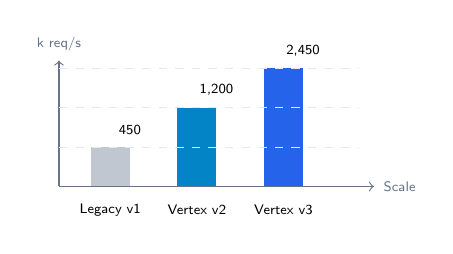
\begin{tikzpicture}[font=\sffamily\tiny]
          % Axes
          \draw[->, color=TextMuted] (0,0) -- (4.0,0) node[right] {Scale};
          \draw[->, color=TextMuted] (0,0) -- (0,1.6) node[above] {k req/s};

          % Bars
          \draw[fill=TextMuted!40, draw=none] (0.4,0) rectangle (0.9,0.5) node[above=1pt] {450};
          \node at (0.65,-0.3) {Legacy v1};

          \draw[fill=SkyAccent, draw=none] (1.5,0) rectangle (2.0,1.0) node[above=1pt] {1,200};
          \node at (1.75,-0.3) {Vertex v2};

          \draw[fill=RoyalAccent, draw=none] (2.6,0) rectangle (3.1,1.5) node[above=1pt] {2,450};
          \node at (2.85,-0.3) {Vertex v3};

          % Grid lines
          \draw[dashed, color=BorderGray] (0,0.5) -- (3.8,0.5);
          \draw[dashed, color=BorderGray] (0,1.0) -- (3.8,1.0);
          \draw[dashed, color=BorderGray] (0,1.5) -- (3.8,1.5);
        \end{tikzpicture}
      \end{tcolorbox}
    \end{column}

    \begin{column}{0.44\textwidth}
      \begin{featurebox}{\faChartLine~ Key Indicators}
        \small
        \begin{compactitemize}
          \item \textbf{P99 Latency:} Reduced from 140ms to \textcolor{TealAccent}{\bfseries 12ms}.
          \item \textbf{Memory:} 45\% reduction via Rust native bindings.
          \item \textbf{High Availability:} Failover under \textbf{1.8s}.
        \end{compactitemize}
      \end{featurebox}
      \vspace*{2pt}
      \begin{tcolorbox}[colback=TealAccent!10,colframe=TealAccent,arc=3pt,top=2pt,bottom=2pt,left=4pt,right=4pt]
        \tiny\color{NavyDark}\textbf{\faRocket~ Result:} 5.4x increase in query capacity.
      \end{tcolorbox}
    \end{column}
  \end{columns}
\end{frame}

% ==========================================
% SECTION 3: ENTERPRISE DEPLOYMENT
% ==========================================
\section{Deployment Strategy}
\label{sec:deployment}

% ------------------------------------------
% SLIDE 11: Section 3 Divider
% ------------------------------------------
\begin{frame}
  \vfill
  \begin{tcolorbox}[
    enhanced,
    colback=NavyDark,
    colframe=SkyAccent,
    boxrule=2pt,
    arc=6pt,
    top=14pt, bottom=14pt, left=14pt
  ]
    {\large\color{SkyAccent}\bfseries SECTION 03}\\[4pt]
    {\huge\bfseries\color{white} Enterprise Deployment Strategy}\\[6pt]
    {\small\color{PageBg!80!white} Migration timeline, risk mitigation, and financial ROI.}
  \end{tcolorbox}
  \vfill
\end{frame}

% ------------------------------------------
% SLIDE 12: Deployment Roadmap Timeline
% ------------------------------------------
\subsection{Roadmap}
\begin{frame}{Implementation Roadmap}{Four-phase structured enterprise rollout}
  \centering
  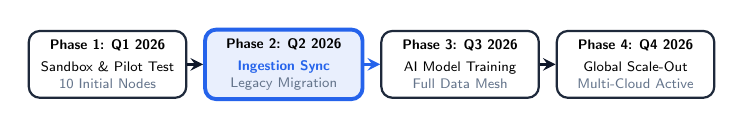
\begin{tikzpicture}[
    node distance=0.3cm,
    font=\sffamily\tiny,
    phase/.style={rectangle, draw=NavySidebar, fill=white, rounded corners=4pt, minimum width=2.0cm, minimum height=0.8cm, align=center, line width=0.8pt},
    active/.style={rectangle, draw=RoyalAccent, fill=RoyalAccent!10, rounded corners=4pt, minimum width=2.0cm, minimum height=0.8cm, align=center, line width=1.4pt}
  ]
    % Nodes
    \node (p1) [phase] {\textbf{Phase 1: Q1 2026}\\[2pt]Sandbox \& Pilot Test\\{\color{TextMuted}10 Initial Nodes}};
    \node (p2) [active, right=0.2cm of p1] {\textbf{Phase 2: Q2 2026}\\[2pt]\textcolor{RoyalAccent}{\bfseries Ingestion Sync}\\{\color{TextMuted}Legacy Migration}};
    \node (p3) [phase, right=0.2cm of p2] {\textbf{Phase 3: Q3 2026}\\[2pt]AI Model Training\\{\color{TextMuted}Full Data Mesh}};
    \node (p4) [phase, right=0.2cm of p3] {\textbf{Phase 4: Q4 2026}\\[2pt]Global Scale-Out\\{\color{TextMuted}Multi-Cloud Active}};

    % Arrows
    \draw [->, >=stealth, line width=1pt, NavyDark] (p1) -- (p2);
    \draw [->, >=stealth, line width=1pt, RoyalAccent] (p2) -- (p3);
    \draw [->, >=stealth, line width=1pt, NavyDark] (p3) -- (p4);
  \end{tikzpicture}

  \vspace*{0.2cm}
  \begin{columns}[T]
    \begin{column}{0.48\textwidth}
      \begin{featurebox}{\faTasks~ Phase 2 Milestones}
        \small
        \begin{compactitemize}
          \item Kafka connector deployment complete.
          \item Dual-write validation (99.99\% parity).
        \end{compactitemize}
      \end{featurebox}
    \end{column}
    \begin{column}{0.48\textwidth}
      \begin{featurebox}{\faExclamationTriangle~ Risk Mitigation}
        \small
        \begin{compactitemize}
          \item Auto-rollback if latency exceeds 50ms.
          \item Parallel execution for zero downtime.
        \end{compactitemize}
      \end{featurebox}
    \end{column}
  \end{columns}
\end{frame}

% ------------------------------------------
% SLIDE 13: Financial ROI & Cost Efficiency
% ------------------------------------------
\subsection{Financial Impact}
\begin{frame}{Financial Impact \& ROI Projections}{Expected cost savings and operational efficiency}
  \begin{columns}[T]
    \begin{column}{0.5\textwidth}
      \small
      \begin{tabular}{lrr}
        \toprule
        \textbf{Cost Category} & \textbf{Legacy} & \textbf{Vertex Projected} \\
        \midrule
        Cloud Compute & \$420,000 & \$260,000 \\{}
        Data Egress & \$180,000 & \$75,000 \\{}
        Maintenance Support & \$150,000 & \$60,000 \\{}
        Compliance Auditing & \$95,000 & \$35,000 \\
        \midrule
        \textbf{Total Annual Cost} & \textbf{\$845,000} & \textbf{\$430,000} \\
        \bottomrule
      \end{tabular}
    \end{column}

    \begin{column}{0.46\textwidth}
      \begin{tcolorbox}[
        enhanced,
        colback=TealAccent!10,
        colframe=TealAccent,
        arc=6pt,
        top=5pt, bottom=5pt, left=6pt, right=6pt
      ]
        {\large\bfseries\color{TealAccent} 49\% Net Cost Savings}\\[2pt]
        {\small\color{NavyDark}\textbf{Annual Savings:} \$415,000}\\[4pt]
        {\tiny\color{TextMain} Projected payback period: \textbf{7.2 months} post rollout.}
      \end{tcolorbox}
      \vspace*{2pt}
      \begin{featurebox}{\faCoins~ Operational Drivers}
        \tiny
        \begin{compactitemize}
          \item Auto-scaling node de-provisioning off-peak.
          \item Compression algorithms reducing footprint 3.2x.
        \end{compactitemize}
      \end{featurebox}
    \end{column}
  \end{columns}
\end{frame}

% ==========================================
% SECTION 4: INTERACTIVE APPENDIX & INDEX
% ==========================================
\section{Interactive Appendix}
\label{sec:appendix}

% ------------------------------------------
% SLIDE 14: Section 4 Divider
% ------------------------------------------
\begin{frame}
  \vfill
  \begin{tcolorbox}[
    enhanced,
    colback=NavyDark,
    colframe=RoyalAccent,
    boxrule=2pt,
    arc=6pt,
    top=14pt, bottom=14pt, left=14pt
  ]
    {\large\color{SkyAccent}\bfseries SECTION 04}\\[4pt]
    {\huge\bfseries\color{white} Interactive Appendix \& Deep Dive}\\[6pt]
    {\small\color{PageBg!80!white} Frequently asked questions and direct slide access index.}
  \end{tcolorbox}
  \vfill
\end{frame}

% ------------------------------------------
% SLIDE 15: Interactive Navigation Index & FAQ
% ------------------------------------------
\subsection{Deck Index}
\begin{frame}[label=deckindex]{Interactive Navigation Directory}{Jump to any presentation topic instantly}
  \begin{columns}[T]
    \begin{column}{0.48\textwidth}
      \begin{featurebox}{\faSitemap~ Section Shortcuts}
        \small
        \begin{enumerate}
          \item \hyperlink{titleframe}{\color{RoyalAccent} Slide 01: Title Page}
          \item \hyperlink{agenda}{\color{RoyalAccent} Slide 03: Executive Agenda}
          \item \hyperlink{sec:vision}{\color{RoyalAccent} Slide 04: Strategic Vision}
          \item \hyperlink{architecture}{\color{RoyalAccent} Slide 06: System Diagram}
          \item \hyperlink{sec:architecture}{\color{RoyalAccent} Slide 08: Core Pillars}
          \item \hyperlink{benchmarks}{\color{RoyalAccent} Slide 10: Benchmarks}
        \end{enumerate}
      \end{featurebox}
    \end{column}

    \begin{column}{0.48\textwidth}
      \begin{featurebox}{\faQuestionCircle~ Frequently Discussed Topics}
        \small
        \begin{compactitemize}
          \item \textbf{Data Privacy:} GDPR compliance?\\
                \hyperlink{sec:architecture}{\beamerbutton{View Security Matrix}}
          \vspace*{2pt}
          \item \textbf{Deployment Hardware:} Specs?\\
                \hyperlink{sec:deployment}{\beamerbutton{View Roadmap \& Specs}}
          \vspace*{2pt}
          \item \textbf{ROI Analysis:} Cost savings?\\
                \hyperlink{sec:deployment}{\beamerbutton{View Financial Impact}}
        \end{compactitemize}
      \end{featurebox}
    \end{column}
  \end{columns}
\end{frame}

% ------------------------------------------
% SLIDE 16: Closing / Q&A Slide
% ------------------------------------------
{
\makeatletter
\setbeamertemplate{sidebar left}{}
\makeatother
\begin{frame}
  \vfill
  \centering
  \begin{tcolorbox}[
    enhanced,
    colback=NavyDark,
    colframe=RoyalAccent,
    arc=8pt,
    width=0.88\textwidth,
    halign=center,
    top=16pt, bottom=16pt
  ]
    {\huge\bfseries\color{white} Thank You!}\\[6pt]
    {\large\color{SkyAccent} Questions \& Discussion}\\[12pt]
    {\small\color{white}\faEnvelope~ contact@nexa-tech.example.com \quad|\quad \faGlobe~ nexa-tech.example.com}\\[10pt]
    \rule{0.5\textwidth}{0.6pt}\\[10pt]
    \hyperlink{titleframe}{\beamerbutton{\faArrowUp~ Return to Cover}} \quad
    \hyperlink{deckindex}{\beamerbutton{\faCompass~ Open Interactive Index}}
  \end{tcolorbox}
  \vfill
\end{frame}
}

\end{document}
